% Section 2 - Middleware in robotics
% Roberto Masocco <roberto.masocco@uniroma2.it>
% April 23, 2025

% ### Middleware in robotics ###
\section{Middleware in robotics}
\graphicspath{{figs/section2/}}

% --- What is middleware? ---
\begin{frame}{What is middleware?}
	\begin{figure}
		\centering
		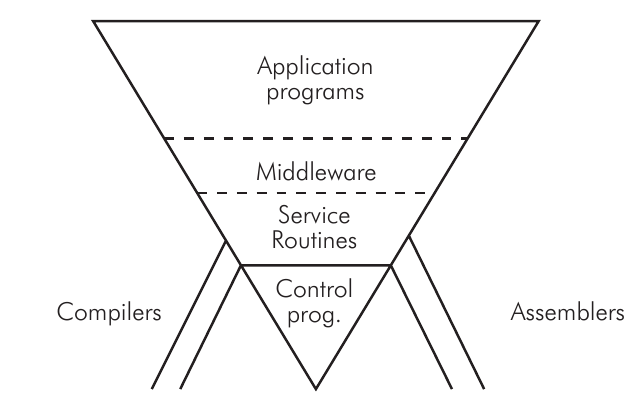
\includegraphics[width=.64\textwidth]{softwarePyramid.png}
		\caption{Software organization in a general-purpose computer system.}
		\label{fig:swpyramid}
	\end{figure}
\end{frame}
\begin{frame}{What is middleware?}
	\begin{block}{Definition of middleware}
		\justifying
		The term \textbf{middleware} identifies a kind of software that offers common services and functionalities to applications in addition to what an operating system usually does.
	\end{block}
	\justifying
	Middleware is usually implemented as \textbg{libraries} that application programmers can use via appropriate \textbg{APIs}.
\end{frame}

% --- Middleware in robotics ---
\begin{frame}{Middleware in robotics}
	\justifying
	New problems arising when developing software for modern autonomous systems:
	\begin{itemize}
		\item integration of \textbg{sophisticated hardware} (microcontrollers, hardware accelerators, SBCs);
		\item \textbg{software} organization and maintenance;
		\item \textbg{communication} (involves both hardware and software!);
		\item debugging and \textbg{testing}.
	\end{itemize}
	\begin{block}{}
		\centering
		Middleware can help to tackle and solve each one!
	\end{block}
\end{frame}

% --- Data Distribution Service ---
\begin{frame}{Data Distribution Service}
	\begin{block}{Definition of DDS}
		The DDS is a \textbf{data-centric communication protocol} used for \textbf{distributed} software application communications, describing APIs and communication semantics between data \textbf{providers} and \textbf{consumers}.
	\end{block}
	\begin{block}{Definition of DDS implementation}
		A DDS implementation is a \textbf{publish-subscribe middleware} that handles communications between \textbf{real-time} systems and software over the \textbf{network}.
	\end{block}
	It is defined by an \href{https://www.omg.org/spec/DDS/About-DDS/}{\color{blue}{\underline{\textbf{{open standard}}}}} maintained by the \textbg{Object Management Group}.
\end{frame}
\begin{frame}{Data Distribution Service}
	DDSs are currently used in automotive, aerospace, military, robotics...\\
	\bigskip
	The open standard defines:
	\begin{itemize}
		\item \textbg{serialization} and \textbg{deserialization} of data packets over supported mediums;
		\item \textbg{security protocols} and cryptographic operations;
		\item enforcing of \textbg{Quality of Service} policies to organize transmissions (specifying things like \textbg{queue sizes}, \textbg{best-effort} or \textbg{reliable} transmissions...);
		\item automatic discovery of \textbg{DDS participants} (\texttt{Discovery Protocol} over \textbg{multicast-IP/UDP}) and transmission of data (over \textbg{unicast-IP/UDP}).
	\end{itemize}
	\bigskip
	Any vendor may add their own extensions to their implementations.
\end{frame}
\begin{frame}{Data Distribution Service}
	An application using the DDS can create one or more \textbg{participants}.\\
	They represent the access point to the DDS network, and embed a \textbg{QoS policy} specifying:
	\begin{itemize}
		\item the \textbg{domain} they belong to (numerical ID);
		\item the \textbg{network interfaces}, \textbg{protocols}, and \textbg{settings} to use.
	\end{itemize}
	\bigskip
	Participants can create \textbg{entities}:
	\begin{itemize}
		\item \textbg{Publishers}, as publication entities, embedding \textbg{DataWriters};
		\item \textbg{Subscribers}, as subscription entities, embedding \textbg{DataReaders};
		\item \textbg{Topics}, as configuration entities with a prescribed \textbg{interface} (packet format).
	\end{itemize}
	Each may enforce a \textbg{QoS policy} specifying its \textbg{desired behavior}.
	\begin{block}{}
		\centering
		\textbf{Communication happens when entities with compatible policies match.}
	\end{block}
\end{frame}
\begin{frame}{Data Distribution Service}
	\begin{figure}
		\centering
		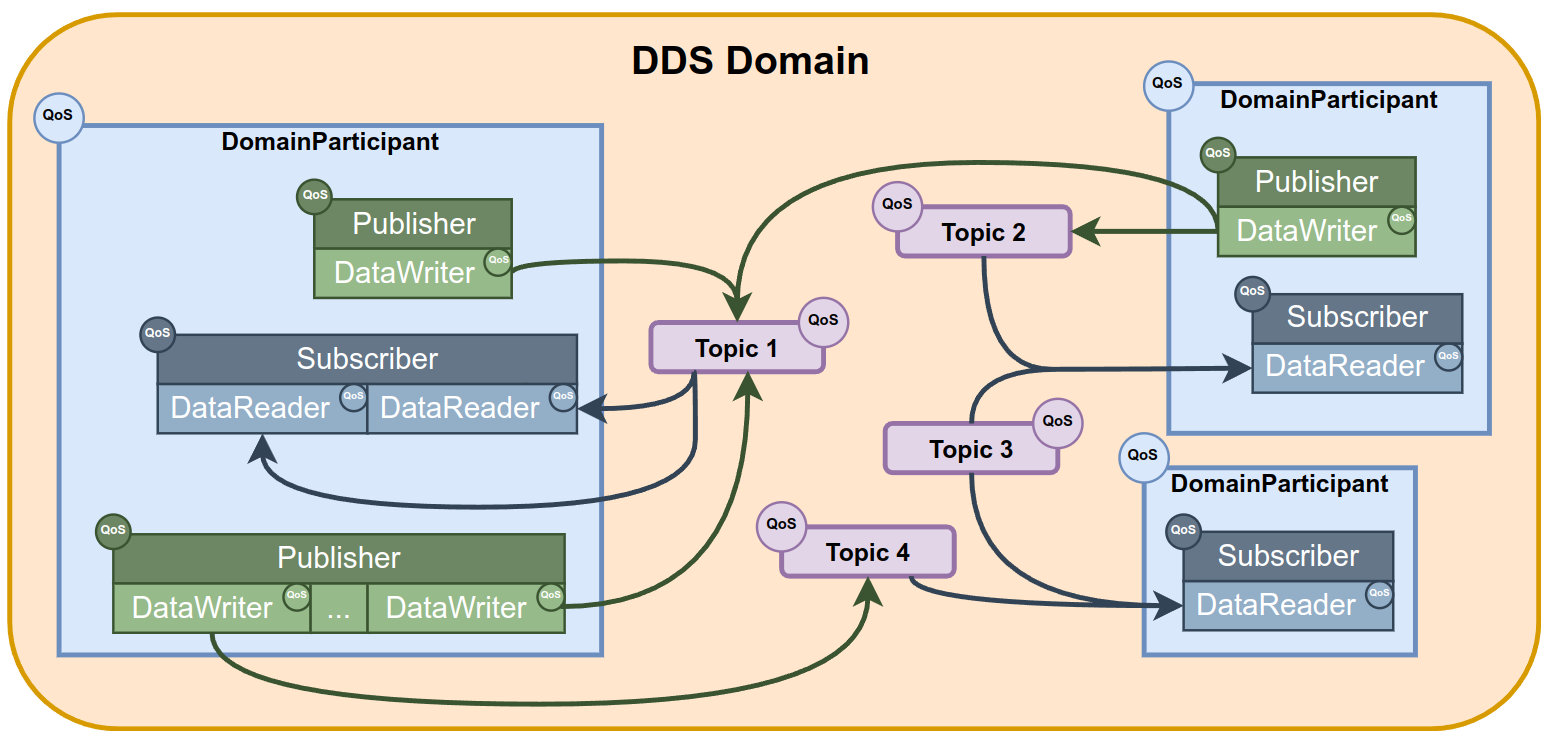
\includegraphics[width=.85\textwidth]{dds_domain}
		\caption{Scheme of a DDS-based network (data space).}
		\label{fig:ddsdomain}
	\end{figure}
\end{frame}
\begin{frame}{Data Distribution Service}{Peeking into the low level}
	Communications are implemented below the DDS layer, by the \textbg{Real-Time Publish Subscribe (RTPS)} protocol.\\
	It defines:
	\begin{itemize}
		\item a \textbg{Discovery Protocol} to automatically find participants over a network in a same domain;
		\item a \textbg{Wire Protocol} to serialize and deserialize data packets;
		\item supported mediums and network protocols;
		\item data exchange semantics: publishing \textbg{changes} of a \textbg{history}.
	\end{itemize}
	\bigskip
	All the entities appear to the application programmer as \textbg{objects} in the code.
\end{frame}
